\documentclass[a4paper,12pt]{article}
% Resten af pakkerne
\usepackage[english, danish]{babel}
\usepackage{csquotes}
\usepackage{float}
\usepackage{flafter}
\usepackage{graphicx}
\usepackage{setspace}
\usepackage{enumitem}
\usepackage{multirow}
\usepackage{lmodern}
\usepackage{amssymb,amsmath}
\usepackage{ifxetex,ifluatex}
\usepackage{lastpage} % Bruges i customtitlepage til at tælle sider
\usepackage[font=small,labelfont=bf]{caption}
\usepackage{lscape}
\usepackage{xargs}
\usepackage{tabularx}

\usepackage{ifthen}

\usepackage{xcolor}
% \usepackage{csvsimple}
\usepackage{longtable}

% Margin
\usepackage{geometry}
\geometry{a4paper,  total={170mm,250mm},
 left=20mm,
 top=30mm}


% New Commands
\newcommand\myworries[1]{\textcolor{red}{#1}} 
\newcommand{\myparagraph}[1]{\paragraph{#1}\mbox{}\\}


% Needs to be the last package included
\usepackage{hyperref}
\hypersetup{
    colorlinks=true,
    linkcolor=black,
    filecolor=magenta,      
    urlcolor=blue,
    citecolor=black,
}


% Linjemellemrum
% \linespread{1.4}
\graphicspath{{./figures/}{../figures/}}

\begin{document}
% Fjerner side tal
\pagenumbering{gobble}
    \renewcommand{\thesection}{\Roman{section}} 
    \renewcommand{\thesubsection}{\thesection.\Roman{subsection}}
    % Forside
    \begin{titlepage}
\begin{center}
% Title
{ \LARGE \bfseries Creditoro \\[0.4cm]}
Et krediteringssystem
\begin{figure}[H]
\centering 
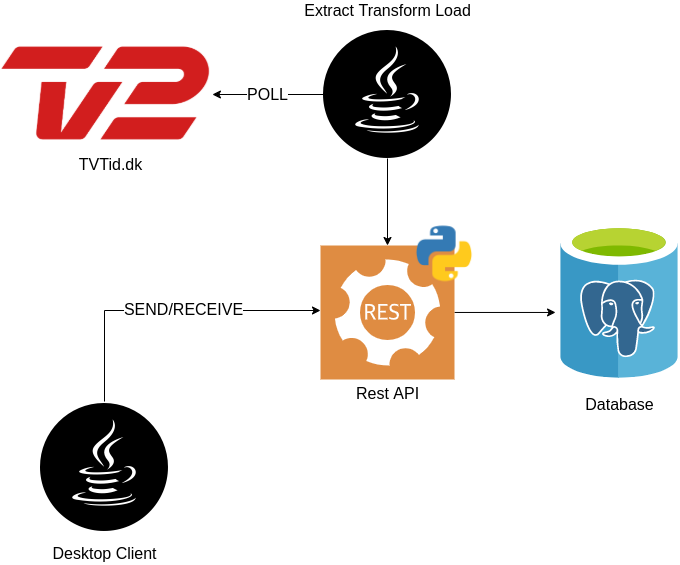
\includegraphics[scale=0.5]{figures/creditoro.png}
\label{figure:creditoro_system}
\end{figure}

Softwareteknologi\\
\vspace{2mm}
Semesterprojekt 2. semester, ST2-PRO\\
\vspace{2mm}
\textbf{Projektperiode:} 01.01.2020 - 29.05.2020 \\
\vspace{2mm}
\textbf{Afleveringsdato:} 29.05.2020 \\

\vspace{7mm}

\textbf{Projektgruppe 06:} \\
\vspace{2mm}
Jakob Rasmussen, jakra19@student.sdu.dk \\
\vspace{2mm}
Kenneth M. Christiansen kechr19@student.sdu.dk \\
\vspace{2mm}
Kevin K. M. Petersen, kepet19@student.sdu.dk \\
\vspace{2mm}
Kristian N. Jakobsen, kjako19@student.sdu.dk \\
\vspace{2mm}
Mathias N. Rasmussen, mara816@student.sdu.dk \\
\vspace{2mm}
Simon Jørgensen, sijo819@student.sdu.dk \\

\vspace{7mm}

\textbf{Vejleder:} Henrik Lykkegaard Larsen, hlla@mmmi.sdu.dk \\

% Bottom of page
\vfill

Syddansk Universitet\\
Det Tekniske Fakultet\\
Mærks Mc-Kinney Møller Instituttet\\
Campusvej 55, 5230 Odense M

\end{center}
\end{titlepage}
    \newpage
    
    % Titelblad 
    \begin{tabular}{@{}l l} 
\textbf{Title:} & Creditoro \\
& \\
\textbf{Institution:} & Syddansk Universitet \\
& Det Tekniske Fakultet, Mærsk Mc-Kinney Møller Instituttet \\
& Campusvej 55, 5230 Odense M \\
& \\
\textbf{Uddannelse:} & Softwareteknologi \\
& \\
\textbf{Semester:} & 2. Semester \\
& \\
\textbf{Semestertema:} & Udvikling af cyber-physical softwaresystemer \\
& \\
\textbf{Kursuskode:} & ST2-PRO \\
& \\
\textbf{Projektperiode:} &  01.01.2020 - 29.05.2020\\
& \\
\textbf{ECTS:} & 10 ECTS\\
& \\
\textbf{Vejleder:} & Henrik Lykkegaard Larsen\\
& \\
\textbf{Projektgruppe:} & 06\\
& \\

\\
\end{tabular}

% VARIABLES
\newcounter{PROD}
\setcounter{PROD} {0}

%%%%


% Jakob Jakob Jakob Jakob Jakob Jakob Jakob Jakob Jakob Jakob Jakob
\ifnum \value{PROD}=1
    
\includegraphics[scale=0.07]{figures/signatures/signatureJR.jpg}
    \vspace{-9.5mm}
\fi
\par\rule{\textwidth}{0.4pt}

Jakob Rasmussen, jakra19@student.sdu.dk\\
% -end- -end- -end -end -end- -end- -end -end -end- -end- -end -end -end-

% Kenneth Kenneth Kenneth Kenneth Kenneth Kenneth Kenneth Kenneth Kenneth

\ifnum \value{PROD}=1
    
\includegraphics[scale=0.3]{figures/signatures/signature_kechr19.PNG}
    \vspace{-5mm}
\fi
\par\rule{\textwidth}{0.4pt}

Kenneth M. Christiansen, kechr19@student.sdu.dk\\
\vspace{3.5mm}
% -end- -end- -end -end -end- -end- -end -end -end- -end- -end -end -end-

% KEVIN KEVIN KEVIN KEVIN KEVIN KEVIN Kevin Kevin Kevin Kevin Kevin Kevin
\vspace{-6.5mm}

\ifnum \value{PROD}=1
    
\includegraphics[scale=0.3]{figures/signatures/signature_kepet19.png}
    \vspace{-8mm}
\fi
\par\rule{\textwidth}{0.4pt}

Kevin K. M. Petersen, kepet19@student.sdu.dk
% -end- -end- -end -end -end- -end- -end -end -end- -end- -end -end -end-

% Kristian Kristian Kristian Kristian Kristian Kristian Kristian

\ifnum \value{PROD}=1
    
\includegraphics[scale=0.04]{figures/signatures/signature_kjako19.jpg}
    \vspace{-9.5mm}
\fi
\par\rule{\textwidth}{0.4pt}

Kristian N. Jakobsen, kjako19@student.sdu.dk\\
% -end- -end- -end -end -end- -end- -end -end -end- -end- -end -end -end-

% Mathias Mathias Mathias Mathias Mathias Mathias Mathias Mathias Mathias

\ifnum \value{PROD}=1
    
\includegraphics[scale=0.120]{figures/signatures/Signatur_mara816.png}
    \vspace{-5mm}
\fi
\par\rule{\textwidth}{0.4pt}

Mathias N. Rasmussen, mara816@student.sdu.dk\\
% -end- -end- -end -end -end- -end- -end -end -end- -end- -end -end -end-

% Simon Simon Simon Simon Simon Simon Simon Simon Simon Simon Simon Simon

\ifnum\value{PROD}=1
    
\includegraphics[scale=0.042]{figures/signatures/signatureSJ.png}
    \vspace{-3.5mm}
\fi
\par\rule{\textwidth}{0.4pt}

Simon Jørgensen, sijo819@student.sdu.dk\\
% -end- -end- -end -end -end- -end- -end -end -end- -end- -end -end -end-


%Bottom of page
%\vfill


\begin{tabular}{@{}l l}
Antal sider:    & \myworries{sider} \\ % \pageref{LastPage} virker ikke mere, da der ikke er sidetal på bilag
Bilag:          & 1 bilag 
\end{tabular}

\vspace{3.5mm}

\begin{footnotesize}

\textbf{Ved at underskrive dette dokument bekræfter hvert enkelt gruppemedlem, at alle
har deltaget lige i projektarbejdet, og at alle således hæfter kollektivt for rapportens indhold.}
\end{footnotesize}
    \newpage

    % Resume
    \section{Resume}
Denne sektion skal indeholde:

\begin{itemize}
    \item Hovedresultater og konklusioner  – hvad kom der ud af arbejdet
\end{itemize}{}

I dette projekt bliver der arbejdet ud fra TV2's problemstilling omhandlende muligheden for at flytte krediteringer fra TV til en anden platform. \myworries{Denne plads kan så udfyldes med andet som fx. reklamer og promoveringer for egne programmer.} Gruppen har valgt at bygge et fuldt funktionelt program, inklusive Rest API og EPG poller. Dertil er gruppen fundet frem til en problemformulering der omhandler udviklingen af et krediteringssystem, hvordan krediteringerne skal gøres tilgængelige samt håndteres. Derudover undersøges det hvordan systemet kan indeholde krediteringerne.
Projektgruppen har valgt at afgrænse projektet ved at lave en prototype til et færdigt program. Ideelt ville systemet også have en webside, dog er dette vurderet til værende udenfor projektets scope.

Overordnet benyttes UP (Unified Process) i hele projektet. UP opdeler hele projektet i 4 faser: \textit{Inceptionsfasen} hvor vigtige krav og kristiske risici identificeres. \textit{Elaborationfasen} hvor en iterativ udvikling af krav, design, analyse og test konstrueres ud fra overordnede kravspecifikationer. \textit{Konstruktionfasen} hvor systemet konstrueres - den faktiske kodeudformning. \textit{Overgangsfasen} hvor det undersøges om systemet er færdigt og ikke har mangler.

I starten af projektets analysefase er et brugsmønsterdiagram, herunder aktørliste og brugs-mønsterliste, udformet. Dette er med til at give et billede af hvordan systemet skal bygges op, samt hvilke aktører der skal kunne interagere med hvilke brugsmønstre. Til prioritering af brugsmønstrene er der foretaget en MoSCoW-analyse.
Til identificering af ikke-funktionelle krav er der brugt metoden FURPS. Her er der sat krav op der omhandler Functionality, Usability, Reliability, Performance og Supportability. For yderligere specificering af ikke funktionelle krav er FURPS+ benyttet - FURPS med ekstra specificerende kategorier med til at opfylde kundens behov.

Til projektstyring benyttes Scrum til at fordele og få overblik over de forskellige opgaver, der opdeles i mindre issues. De forskellige arbejdsopgaver inddeles i sprints som forløber sig over en given periode - i dette projekts tilfælde to uger.

\myworries{Hovedresultater og konklusioner}



    \newpage
    
    % Forord
    \section{Forord}
Denne sektion skal indeholde:

\begin{itemize}
    \item Hensigten med rapporten, målgruppe, forhistorie, anerkendelser
\end{itemize}{}

    \newpage

    % Indholdsfortegnelse
    \tableofcontents
    \newpage
    
    % Læsevejledning
    \input{tex/vi_læsevejledning}
    \newpage
    
    \section{Redaktionelt}

    \newpage
    
    % Start counting from this line
    \pagenumbering{arabic}
    \setcounter{page}{1}

    \renewcommand{\thesection}{\arabic{section}} 
    \renewcommand{\thesubsection}{\thesection.\arabic{subsection}}
    \setcounter{section}{0}
    % Introduktion
    \section{Introduktion}

Når et program bliver broadcasted på en TV station, skal krediteringer vises. Dette gøres i slutningen af programmet, i maksimalt 30 sekunder. Det betyder, at der ikke altid er tid til at vise alle krediteringer, og derfor prioriteres de før de vises. \\
Hvis de 30 sekunder for hvert program kan frigøres, kan danske TV stationer bruge tiden på at vise noget andet, som f.eks. reklamer. Derved kan TV 2 øge deres årlige indtægter med op til 60 millioner kroner. \\
TV 2 har brug for et system, der kan administrere krediteringer for programmer produceret i Danmark. Hertil skal der kunne tilføjes nye krediteringer i systemet for nye produktioner, samt det skal være muligt at kunne søge efter eksisterende krediteringer. Det skal være muligt at kunne se hvilken rolle en given person har haft i en produktion, da denne person kan have haft flere forskellige roller på flere forskellige produktioner.

\subsection{Projektrammer}
Denne sektion har til formål at opridse rammerne for projektet, samt hvilket område projektgruppen arbejder indenfor.

\subsubsection{Krav til Projektet}
Systemet skal så vidt muligt skrives i programmeringssproget Java. \\
Krediterings-data skal lagres i en database, og i dette projekt skal den brugte database være SQL baseret. Der skal bruges PostgreSQL.\\
Systemet forventes ikke at være et færdigt system, men en række forslag til løsninger der opfylder systembehovet. Forslagene skal inkludere:

\begin{itemize}
    \item Krav
    \item Analyse
    \item Design
    \item Implementering
    \item Test
\end{itemize}

\noindent
Producere der kan tilføje og redigere i krediteringerne, skal kun have mulighed for at redigere i de produktioner, de selv ejer.\\
Det forventes at krediteringssystemet er kompatibelt med andre systemer (f.eks. fra Stofa, YouSee etc.).

\subsubsection{Tidsplan}
Tidsplanen har til formål at skabe overblik og styring over projektet. 
Den giver gruppemedlemmerne et overblik over, hvornår de forskellige dele af projektet skal starte og slutte, og derved bliver det hurtigt klart hvis tidsplanen skrider. \\

\begin{landscape}
    \begin{figure}
        \centering
        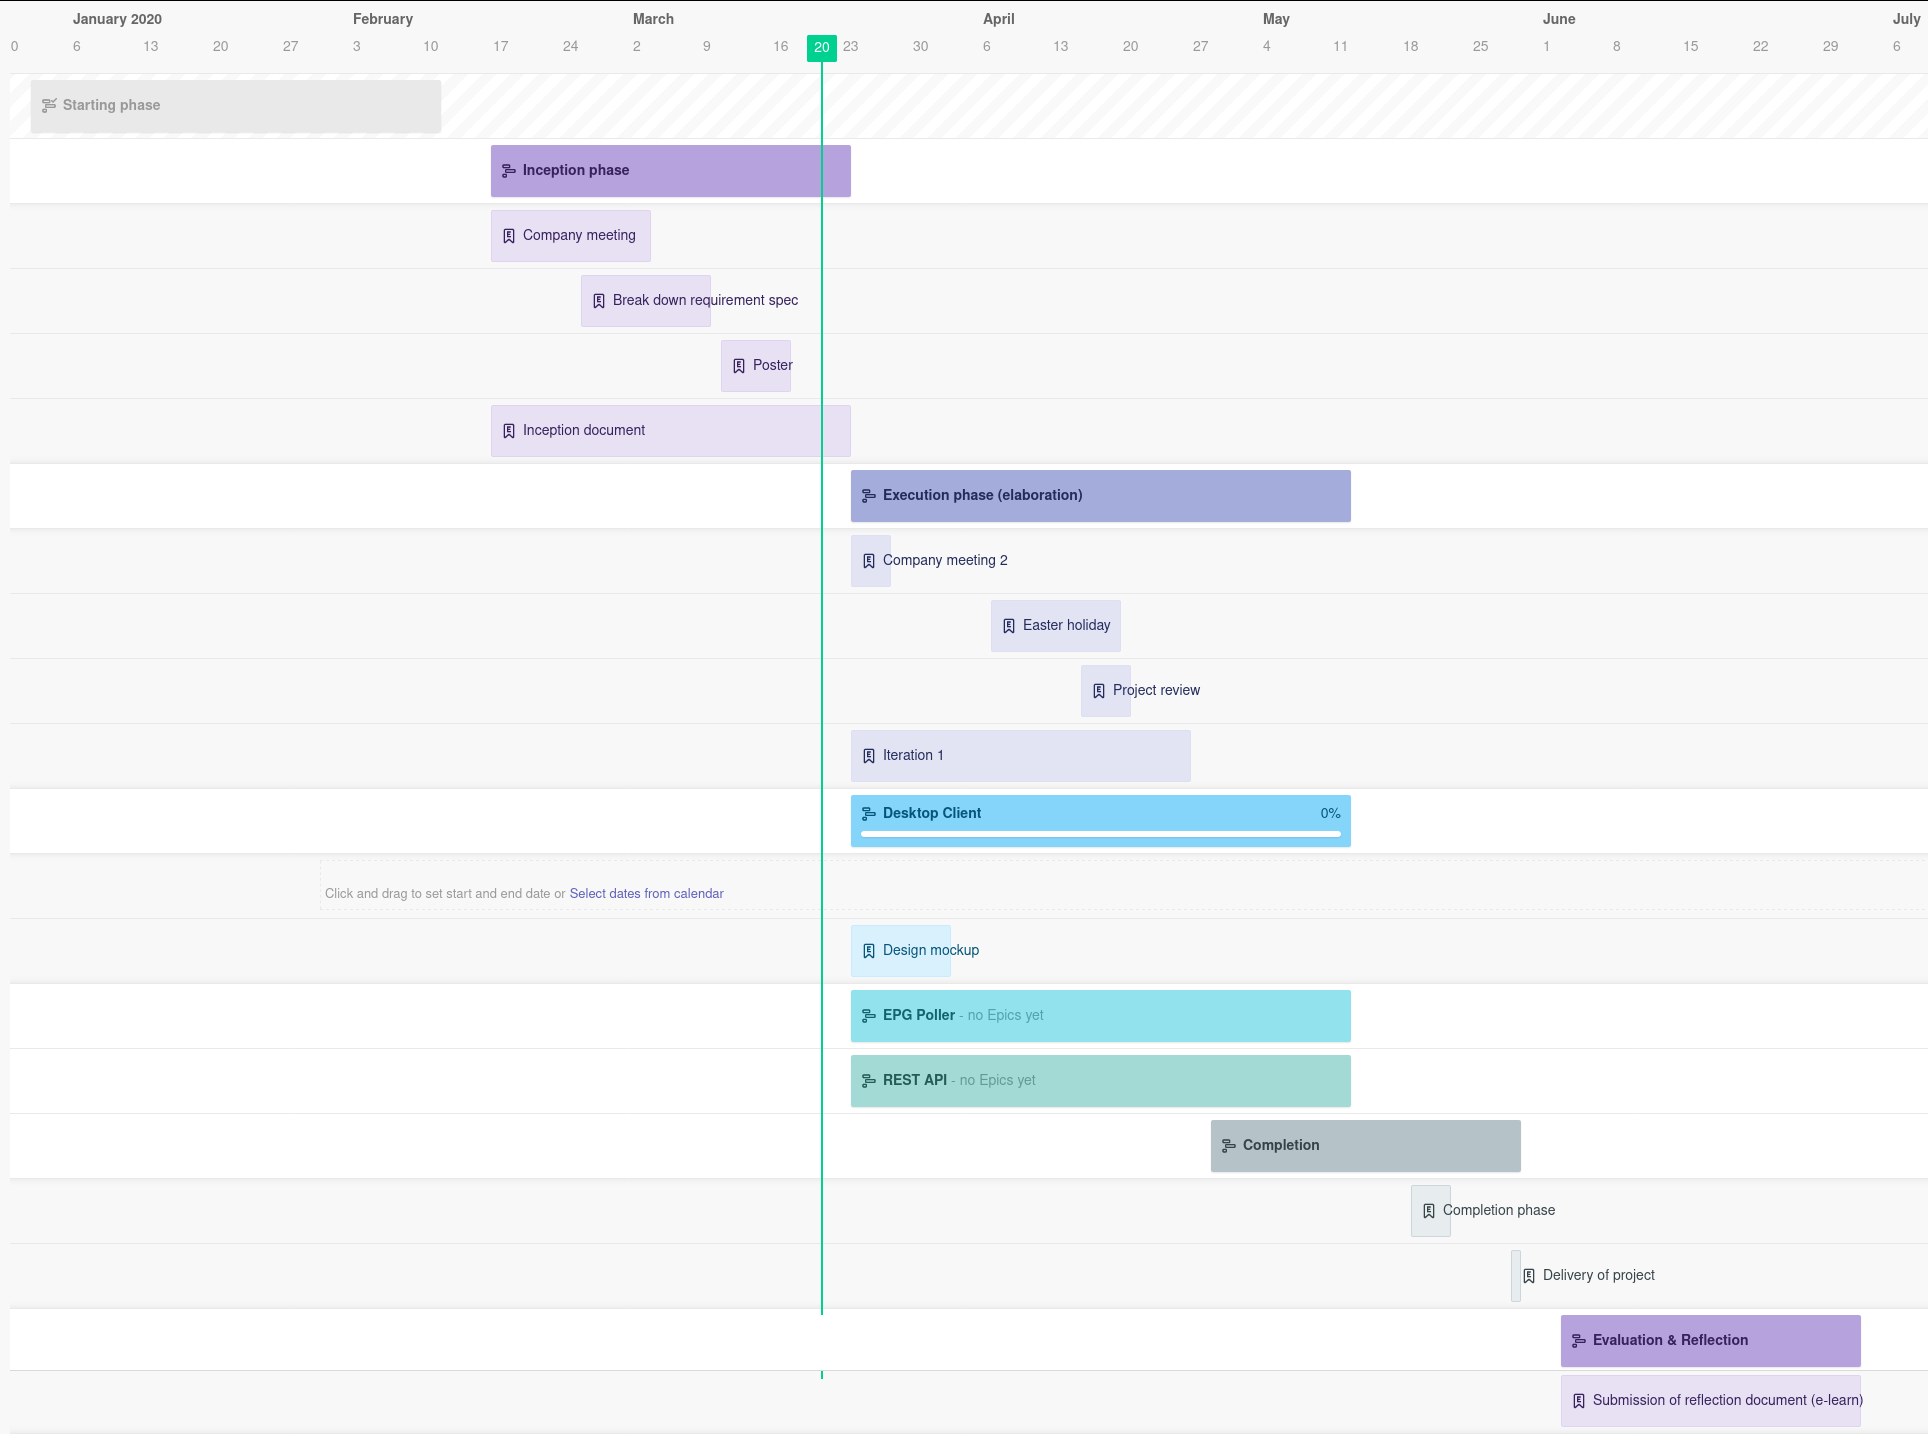
\includegraphics[scale=0.30]{figures/grantt_udvidet.png}
        \caption{Tidsplan for projektet}
        \label{fig:gantt}
    \end{figure}{}
\end{landscape}

% PRE review
% \subsubsection{Hvad ligger uden for projektrammen}
% Der forventes ikke at der laves et produktionsparat system, men et system der kan bruges som et værktøj af TV2. % PRE review: Det er derfor uden for systemets omfang (scope) at lave en REST API.

\subsection{Formål med Inceptionsfasen}
Formålet med inceptionsfasen er at fastlægge systemets omfang, der bliver udformet en overordnet kravspecifikation, kravene prioriteres og metoderne i elaborationsfasen beskrives. Dette sker gennem en nærmere undersøgelse af problemstillingen, indsamling af information og under kundemøder hvor kravene indsamles (eliciteres).\\

\noindent
Målene for inceptionsfasen kan således opstilles i punktform:
\begin{itemize}
    \item At gennemføre kravudvikling
    \item At identificere kritiske risici
    \item At fastlægge projektets metoder i elaborationsfasen
\end{itemize}

\subsection{Problemanalyse}
% PRE review: Hvordan kan vi udvikle et samlet krediteringssystem, der giver mulighed for at erstatte rulletekster efter et endt program?

\subsubsection{Igangsættende Problem}
TV2 ønsker at frigøre 30 sekunders krediterings tekster efter hvert program, så de i stedet kan bruge tiden på at vise reklamer. Problemet består i at disse krediterings tekster, så skal vises på en anden platform.\\

\noindent
I tabel \ref{table:kravFraCase} ses kravene fra TV2's projektcase:

% Oversæt gerne højre kolonne til dansk :-)
\begin{longtable}{|p{12cm}|p{4cm}|}
\hline
\textbf{Beskrivelse} & \textbf{Type} \\
\hline
“Vi har brug for  et krediterings system der kan  håndtere  dansk TV content” 
& En vag opgave \\

\hline
"Dette inkluderer muligheden for at oprette nye krediteringer i systemet, når en ny produktion bliver lavet, samt at have mulighed for at søge efter en given produktion og få en liste af krediteringer, forbundet til denne. Det burde også være muligt at se hvilken rolle en given person har haft i en produktion, eftersom en person kan have flere forskellige roller i forskellige produktioner."
& Ønske om en bestemt løsning \\

\hline 
"Producers/TV-stationer burde være i stand til at redigere krediteringer for programmer/produktioner de ejer. De burde også være i stand til at redigere disse produktioners ID. Systemadministratorer skal kunne vedligeholde (oprette, læse, opdatere og slette) personer, krediteringer og personer."
& Ønske om en bestemt løsning \\

\hline
"Til slut skal systemet kunne offentliggøre en service som andre systemer kan bruge. Disse systemer kan f.eks. være en hjemmeside eller en applikation. Disse andre systemer skal også kunne bruge API'et, så data'et kan blive brugt i allerede eksisterende systemer (såsom TVTID.dk - TV 2's TV-Guide)."
& Ønske om en bestemt løsning \\

\hline
"En form for adgangskontrol skal implementeres, til de beskyttede dele af systemet (oprettelse, opdatering, slettelse, osv. af data)
& Ønske om en bestemt løsning \\

\hline
"Der skal være en offentligt tilgængelig del af systemet, hvor det er muligt at se krediteringer uden at logge ind."
& Ønske om en bestemt løsning \\

\hline
“Nuværende løsning er begrænset til 30 sekunder, og dermed kan alle krediteringerne ikke altid vises i praksis” 
& Et problem \\

\hline
\caption{Krav fra TV2s projektcase}
\label{table:kravFraCase}
\end{longtable}

% -----------------------------------------------------------------------------------------------------
\subsubsection{Identifikation af Problemet}
Som det er nu bliver krediteringer vist i slutningen af et program. Ifølge reglerne for visning af krediteringer, må krediteringer ikke vises mere end 20 sekunder for produktioner under 60 minutter, og 30 sekunder for produktioner over 60 minutter. Dette giver en del problemer. For det første betyder den begrænsede varighed, at ikke alle medarbejdere kan krediteres. Dette ender ud i at der skal prioriteres i krediteringerne, før de bliver vist på TV. Derved får alle medarbejdere ikke den anerkendelse de burde.
Hvis krediteringer flyttes til et eksternt system, og derved ikke bliver vist på TV, kan man undgå at skulle prioritere. Alle kan derved få den fortjente kredit. Derudover vil det også give mulighed for at vise noget andet, som f.eks. reklamer eller promoveringer for andre programmer (red: eget indhold).
\footnote{\href{https://www.dr.dk/NR/rdonlyres/00221a7b/dpikscstjptklixxdnjgywgeuakhwpog/DR_kreditmanual_050810.pdf}{DR’s krediteringsregler for TV}}
% brug bibliography. show me the way

\noindent
Et sådan eksternt system vil også hjælpe med oprettelsen af nye krediteringer, ved at gøre processen hurtigere og nemmere, samt mere overskueligt. Dertil har gruppen valgt at arbejde med samtlige/alle problemstillinger givet af TV2 i tabel \ref{table:kravFraCase}, og lave en prototype til et funktionsdygtigt system. Angående valget med at arbejde med samtlige problemstillinger præsenteret af TV2, har gruppen konkluderet det som værende realistisk jævnfør figur \ref{fig:gantt}. Denne prototype vil kunne bruges som et udkast til et endeligt system.

\subsection{Problemformulering \& Afgrænsning}
\textit{Hvordan kan vi udvikle et samlet krediteringssystem, der giver mulighed for at erstatte rulletekster efter et endt program?}

\begin{enumerate}
    \item Hvem skal kunne håndtere krediteringer?
    \item Hvordan skal krediteringerne gøres tilgængelige, og hvordan skal seerne refereres dertil?
    \item Hvordan kan man oprette et system som kan indeholde krediteringer?
\end{enumerate}

\noindent % afgrænsning
Projektgruppen har valgt at afgrænse dette projekt, ved at konstruere en prototype til et system.
% Indsat post review. 

\noindent % Det vi har med:
Projektgruppen har valgt at lave et system der ligger tæt op ad det oprindelige foreslag fra TV2s projektcase. Dette indebærer alle kravene i tabel \ref{table:kravFraCase}.
\begin{figure}[H]
\centering
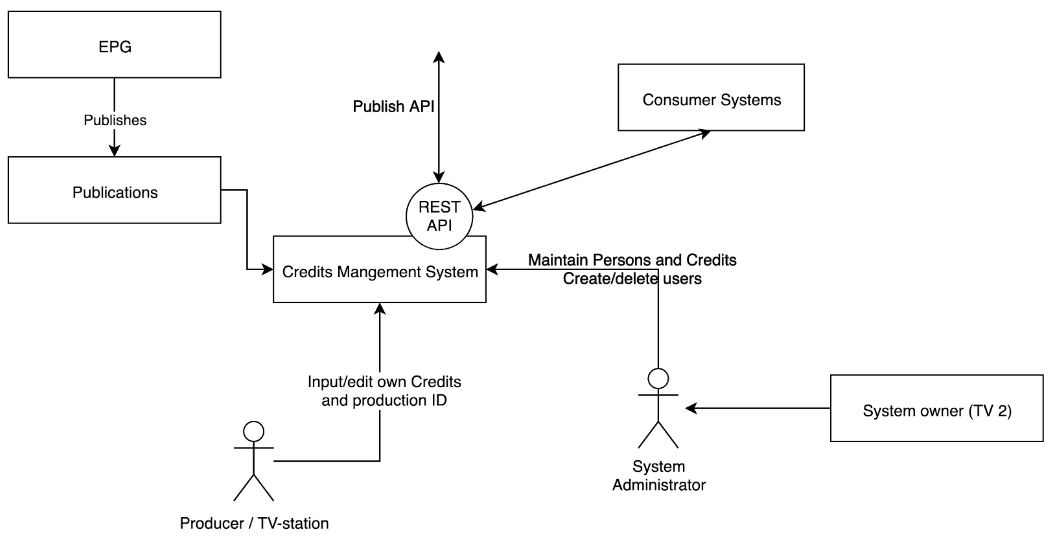
\includegraphics[scale=0.3]{figures/tv2_system.png}
\label{fig:tv2_system}
\caption{Foreslag til systemtegning - © TV2}
\end{figure}
% Indsæt figur af deres oprindelige systemtegning?

\noindent % Det vi vælger fra:
I et produktionsklart system vil det være ideelt at have en webside, men dette har vi konkluderet som værende uden for projektet.
    \newpage
    
    % Faglige vidensgrundlag
    % Fagligt Videngrundlag ----------------------------------------------------------------------------
\section{Faglige Vidensgrundlag}
Dette afsnit har til formål at dækker over den faglige viden gruppen skal have, for at kunne udføre projektet.

\subsection{JAVA}
At have kendskab til Java er en vigtig forudsætning for udarbejdelsen af projektet. Systemet vil hovedsageligt blive programmeret i sproget Java. Det faglige niveau svarer til 2. semesterstuderende på Softwareteknologi. Dette indebærer blandt andet forståelse af JavaFX og Scenebuilder.
Arbejdet med Java i projektet forudsætter derudover forståelse for basale programmeringsprincipper og forståelse for det objektorienterede programmeringsparadigme. 

\subsection{Python}
Et grundlæggende kendskab til Python kræves for at kunne forstå - samt implementere REST Api'et.

\subsection{Database}
Systemet vil indeholde en lang række data, som skal lagres i en database. Det er derfor nødvendigt at have forståelse for databaser, databasestrukturer, relationelle SQL-databaser og SQL-queries. Databasen der vil blive benyttet i projektet er PostgreSQL, en basal viden om databasesproget/programmeringssproget SQL er derfor nødvendig. 
Al nødvendig viden er givet i SDU's 'Data Management' kursets pensum.

\subsection{Ubuntu \& Docker}
En basal forståelse for Ubuntu (eller andet Linux baseret distro) og Docker kræves for opsætning af REST Api'et og databasen.

\subsection{Relevante Eksisterende Løsninger}
\textbf{IMDb} \\
IMDb (Internet Movie Database) er en online database bestående af film, serier, medvirkende m.m. Man har mulighed for at søge efter informationer ved at referere til blandt andet førnævnte titler. IMDb har også et ratingsystem, der gør det muligt at bedømme film, serier etc.\\
\textbf{Rotten Tomatoes} \\
Rotten Tomatoes er på lige fod med IMDb, en database for film, serier, medvirkende m.m. Man kan på Rotten Tomatoes også søge information. Rotten Tomatoes distancerer sig fra IMDb, ved både at tage ratings fra sine brugere og et panel af anmeldere. 
    \newpage
    
    % Metode
    \section{Metode}
    \newpage
   
    % Hovedtekst
    \section{Hovedtekst}

\input{tex/4_1_detaljerede_brugsmønstre}
\newpage

\section{Supplerende krav}

Her bruges FURPS for supplerende krav.
\begin{table}[H]
    \centering
    \begin{tabular}{|p{3cm}|p{13cm}|}
    \hline
    \textbf{FURPS}           &    \textbf{Krav} \\
    \hline
    %What the customer wants! Note that this includes security-related needs.
    Functionality           & Skal kunne kreditere produktionsroller som er angivet af DRs Krediteringsregler \\
                            & Skal overholde GDPR \\
    \hline
    % How effective is the product from the standpoint of the person who must use it? Is it aesthetically acceptable? Is the documentation accurate and complete?
    Usability       & Systemet skal kunne understøtte flere sprog \\
    \hline
    % What is the maximum acceptable system downtime? Are failures predictable? Can we demonstrate the accuracy of results? How is the system recovered?
    Reliability     &  Hvis serveren til systemet genstarter, startes del-systemerne igen automatisk. Der vil ikke være behov for at ligge systemet ned regelmæssigt for at kunne foretage backup. \\
    \hline
    % How fast must it be? What's the maximum response time? What's the throughput? What's the memory consumption?
    Performance     &  Databasen skal kunne håndtere 10000 nye brugere - samt 15000 krediteringerer årligt i 25 år, uden at ofte brugte kald til REST Api'et bliver sløvt (reponsetid på mere end 300 ms) \\
    \hline
    % Is it testable, extensible, serviceable, installable, and configurable? Can it be monitored?
    Supportability  &  Systemet vil indeholde unit tests, og komme med en rapport over hvor stor en procendel der er dækket af dette. % Hvis der er mere tid kan vi indrage integrations tests?
    %Centraliseret logning (Elastic search, eller blot centraliseret system log?)
    Systemet vil blive forbundet til det centraliserede fejllognings system \texttt{Sentry}.
    Systemet er installerbart vha. Docker via Docker-compose. % (så vi blot kan sige docker-compose up -d for at få systemet op).
    Det vil være muligt at konfigurere system indstillinger via en \texttt{.env} (miljø) fil.
    En opsætningsguide vil være at finde sammen med kildekoden. 
    \\ \hline
    % The + reminds us of a few additional needs that a customer could have:
    % fx. Design constraints, Implementation requirements, interface requirements or physical requirements.
    \end{tabular}
    \caption{FURPS}
    \label{tab:furps}
\end{table} 

\myworries{Følgende skal overvejes:}

\begin{itemize}
    \item Usability: Responsive UI
    \item Perfomance: The system should be able to handle 5000 concurrent users within a minute.
\end{itemize}

\newpage

\input{tex/4_1_brugsmønsteranalyse}
\newpage

\input{tex/4_2_brugsmønsterrealisering}
\newpage

    \newpage
   
    % Procesdokumenter
    % \section{Procesdokumenter}

\subsection{Gruppekontrakt}
\paragraph{Forventninger \& Mål}
\begin{itemize}
    \item Forventer alle yder sin del
    \item Der forventes der bliver lagt en passende mængde tid i arbejdet. fx 2 timer er ikke nok pr. Uge.
    \item Ambitionsniveauet er alle gør sit bedste, så vi i sidste ende føler at vi har gjort en hel hjertet indsats.
\end{itemize}

\paragraph{Gruppens Arbejdstider}
\begin{itemize}
    \item Kører med det akademiske kvarter
    \item Vi mødes kl 08, her under gælder det akademiske kvarter.
    \item Sygdom Læge eller lignende, skal man informere gruppen. Inden kl 08 på dagen.
    \item Gruppen forkrost pause, efter vejleder møde. 30 min frokost pause.
    \item Hvis der gives hjemme arbejde, skal det laves til det aftalte tidspunkt.
    \item Går hjem kl 14:00 medmindre andet aftales.
\end{itemize}

\paragraph{Gruppemøder}
\begin{itemize}
    \item Gruppen mødes fast.
    \item Møder forgår som udgangspunkt på SDU hver tirsdag, men der er muligheder for at kunne aftale andet i løbet af projektet hvis der er brug for det.
    \item Hvis man kommer for sent, kan der pålægges en straf, med mindre oversagen kan beggrundes.
    \item Straffen kan være: spiselige eller drikkelige ting. 
    \item Hvis man ikke dukker op til møderne, skal det meddeles til medlemmerne helst inden vi mødes kl 08:00.
	\begin{itemize}
	    \item Hvis man gentagende gange udebliver, skal det løses internt i gruppen, ellers skal vejlederen inddrages.
	\end{itemize}
    \item Hyggesnak godtages i passende mængder, men tiden skal bruges fornuftigt.
\end{itemize}

\paragraph{Organisering af møder}
\begin{itemize}
    \item  Ordstyrer bliver valgt på dagen.
    \item  Referent bliver valgt på dagen.
    \item  I Gruppen vil man forsøge at skrive referat og logbog samlet.
    \begin{itemize}
        \item Der er en der har hoveddeansvaret for referat og logbog, resten supplere til dem.
    \end{itemize}
    \item  Alle deadlines og indbyrdesaftaler overholdes og hvis det ikke er muligt, skal det skrives ind logbogen.
    \item  Hver mødes skal skrives ind i logbogen og det vil sige  dagsorden, eventuelt problemer osv.
\end{itemize}

\paragraph{Arbejdsindsats}
\begin{itemize}
    \item Der bliver aftalt fra gang til gang hvordan der skal arbejdes.
    \item Pair programmering
    \item GitHub: Merge request uden reviews
\end{itemize}

\paragraph{Vejledermøde}
\begin{itemize}
    \item Der holdes vejleder møde hver eneste uge
    \item Der sendes senest en møde indkaldelse med lokale, link til dagsorden, samt materialer, via outlook til vejlederen senest senest 23.59 Fredag.
\end{itemize}

\paragraph{Kursusdeltagelse}
\begin{itemize}
    \item Det forventes af hver gruppemedlem har læst op og fået styr på de emmer, vi arbejder med, inden møderne og arbejdsdagene.
    \item Der skrives så hvidt muligt kommentar i koden.
    \begin{itemize}
        \item Kommentarende skrives på engelsk.
    \end{itemize}
\end{itemize}

\paragraph{Brug \& Revision Samarbejdsaftalen}
\begin{itemize}
    \item Samarbejdsaftalen tages i brug løbende.
    \item Aftalen tages i brug ved konflikter.
    \item aftalen kan blive revidereeget løbende, hvis der er behov for det.
    \begin{itemize}
        \item Den nye aftale skal godkendes af alle medlemmer.
    \end{itemize}
\end{itemize}

\paragraph{Værktøjer}
\begin{itemize}
    \item Primære kommunikationsmidler
    \begin{itemize}
        \item Tekst: Discord, Mail
        \item Samtaler: Discord
    \end{itemize}
    \item Github
    \begin{itemize}
        \item Kodebibliotek
        \item Logbog
        \item Referat
        \item Aftaler
    \end{itemize}
    \item Fildeling
    \begin{itemize}
        \item OneDrive
    \end{itemize}
\end{itemize}

\myparagraph{Belbien Teamroller}
Belbien teamroller se i billag side \pageref{table:belbien} tabel \ref{table:belbien} 

\paragraph{Kontakt Oplysninger}
\begin{itemize}
    \item Jakob Rasmussen
    \begin{itemize}
        \item jakra19@student.sdu.dk
        \item 52 40 56 62
    \end{itemize}
    \item Kenneth Munk Christiansen
        \begin{itemize}
        \item Kechr19@student.sdu.dk
        \item 28 67 66 78
    \end{itemize}
    \item Kevin Kamper Meejach Petersen
        \begin{itemize}
        \item kepet19@student.sdu.dk
        \item 50 30 88 58
    \end{itemize}
    \item Kristian Nymann Jakobsen
        \begin{itemize}
        \item kjako19@student.sdu.dk
        \item 22 80 53 26
    \end{itemize}
    \item Mathias Nickolaj Rasmussen
        \begin{itemize}
        \item mara816@student.sdu.dk
        \item 28 12 89 41
    \end{itemize}
    \item Simon Jørgensen
        \begin{itemize}
        \item sijo819@student.sdu.dk
        \item 42 83 25 60
    \end{itemize}
\end{itemize}

\newpage
\subsection{Vejlederkontrakt}
\begin{itemize}
    \item Der skal laves en gennemgang og dagsorden til hvert vejledermøde. Det skal sendes til vejleder senest fredag kl. 23.59.
    \item Alt skal så vidt muligt holdes i GitHub.
    \item Vejleder læser alle dokumenter og materialer igennen, vi sender, og dette skal gøres før vejledermødet.
    \item Vi tager ansvar for eget studie, og står selv for fremmøde til undervisning.
    \item Vejledermøde er som udgangspunkt hver tirsdag kl. 11.15.
    \begin{itemize}
        \item Hvis tidspunktet ændres aftales det med vejleder via mail.
    \end{itemize}
    \item Vejleder gør gruppen opmærksom på om gruppearbejdet er på afveje, samt at eventuelle deadlines ikke overholdes, så gruppen kan nå i mål uden konflikter.
    \item Vejleder giver besked via mail hvis han bliver forhindret i at afholde vejledermøde, eller hvis tidspunktet bliver ændret.
    \item Hvis gruppen skulle blive utilfreds med vejleders indsats, skal dette håndteres hurtigst muligt.
    \item Hvis gruppen kommer på afveje i forhold til samarbejdsaftalen, skal vejleder være i stand til at vejlede gruppen gennem eventuelle konflikter.
\end{itemize}

\newpage
\subsection{Belbin Gruppeprofil}
\begin{table}[ht]
\centering
\begin{tabular}{|p{3cm}|p{2cm}|p{2cm}|p{2cm}|}
\hline
\textbf{Teamrolle} & \textbf{Navn} & \textbf{Navn} & \textbf{Navn} \\ \hline
Idémand & Mathias & Kevin & Jakob \\ \hline
Kontaktskaber & Kevin & Kenneth & \\ \hline
Koordinator & Kristian & Mathias &  \\ \hline
Opstarter & Simon & Mathias &  \\ \hline
Analysator & Jakob &  &  \\ \hline
Formidler & Kevin & Kristian &  \\ \hline
Organisator & Kenneth & Simon &  \\ \hline
Afslutter & Kenneth & Simon & \\ \hline
Specialist & Kristian & Jakob & \\ \hline
\end{tabular}
\caption{Belbien Teamroller}
\label{table:belbien}
\end{table}
    % \newpage
    
    % Bilag
    \appendix % Bruges til bilag, så den laver bilag indholdfortegnelse og overskrifter
    \documentclass[../report.tex]{subfiles}
\begin{document}

\section{Appendices}

Bilag

\end{document}
    

    % bibliography empty
    \newpage
    \bibliographystyle{apalike}
    \bibliography{appendices/bibliography.bib}
\end{document}
